Para este tema es importante tener claros varios conceptos que vamos a ir definiendo y explicando poco a poco.

\begin{defn}[Middleware]
Conjunto de aplicaciones encargadas de enlazar los componentes de un sistema distribuido.
\end{defn}

\section{Network Operating System (NOS)}
Este conjunto de aplicaciones está dividido en el protocolo específico del servicio con el que estamos trabajando (ODBC, HTTP, SMTP...), el protocolo de transporte (TCP/IP) y una capa intermedia llamada Network Operating System (NOS)}.

\begin{defn}[Network Operating System]
Es una extensión del sistema operativo que proporciona transparencia al cliente, para que éste realice las llamadas como si fueran locales.
\end{defn}

Algunas de las maneras de proporcionar transparencia del NOS según \concept{RM-ODP} (Open Distributed
Processing Reference Model) son
\begin{itemize}
\item Ubicación: Ocultar dónde reside cada recurso (y permite que éste se mueva, incluso mientras está siendo utilizado).
\item Persistencia: Ocultar tanto la activación y desactivación de objetos como sus fallos y recuperaciones mediante la replicación.
\item Concurrencia: Ocultar la utilización de recursos concurrentes.
\item Prestaciones: Escalar el tamaño y reconfigurar el sistema para mejorar sus prestaciones según varía la carga de trabajo.
\item Espacio de nombres:
\item SSO: Single Sign On - Un único usuario y contraseña para todo el sistema.
\item Tiempo: Todos los componentes deben estar sincronizados.
\item Protocolos: Idéntica interfaz de programación para todos los protocolos de transporte.
\end{itemize}

Debido a que la representación interna de los datos es dependiente del ordenador (hardware o sistema operativo) es necesario definir un mecanismo para que, independientemente de la plataforma, la comunicación sea posible. Algunos métodos son utilizar estándares de \textbf{codificación de caracteres} (ISO-8859-1,UTF-8), \textbf{XML}, sistemas propios de aplicaciones (\textbf{RPC,XDR}) o un estándar \textbf{Abstract Synyax Notation} (con una gramática y reglas para codificar los datos).


\section{Servicios de transporte}

Una vez hablado del NOS, vamos a ver unos conceptos de  servicios de transporte del middleware.

Lo primero es recordar que hay 2 modelos de interacción, \textbf{síncrono} o \textbf{asíncrono}. Además de estos modelos, las interacciones pueden ser de tres tipos.
\begin{itemize}
	\item \textbf{R:} Petición. (El cliente hace una petición sin esperar respuesta, por ejemplo para cerrar la conexión)
	\item \textbf{RR:} Petición → Respuesta.
	\item \textbf{RRA:} Petición → Respuesta → ACK.
\end{itemize}

\subsection{API directa}

\begin{defn}[APIs directas]
API viene de \textit{Application Programming Interface} (Interfaz de programación de aplicaciones).

La utilización de APIs directas es la utilización de una interfaz de programación para acceder a unos servicios (proporcionados por la aplicación).
\end{defn}

Habitualmente son servicios de nivel de transporte o sesión. La ubicación de extremos no es transparente para el programa, ya que necesitas saber dónde está la interfaz para poder utilizarla. Para ver un ejemplo de API, consultar: \href{https://apigee.com/OneDrive/embed/console/OneDrive}{API de OneDrive}.

\subsection{Sockets}

Son la leche porque proporcionan mucha transparencia: podemos comunicarnos entre procesos sin tener ni idea de nada, simplemente es como escribir en un fichero (de hecho, si recordamos de Redes II un socket es directamente un descriptor de fichero en Linux).

Aunque ya deberíamos saberlo, incluimos un par de esquemas (sacados de las transparencias) en los que vemos cómo establecer una comunicación orientada a conexión (\ref{SocketConexion}) y una comunicación no orientada a conexión (\ref{SocketNoConexion})


\begin{figure}[hbtp]
\centering
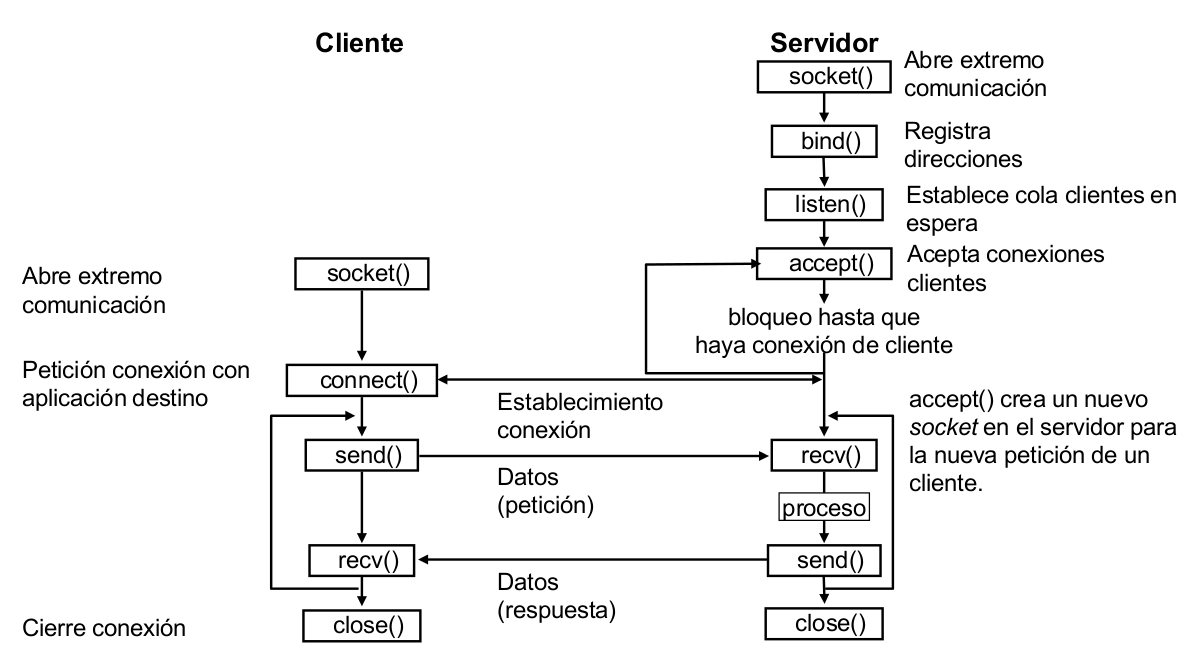
\includegraphics[width=1\textwidth]{img/SocketConexion.png}
\caption{Comunicación orientada a conexión.}
\label{SocketConexion}
\end{figure}

\begin{figure}[hbtp]
\centering
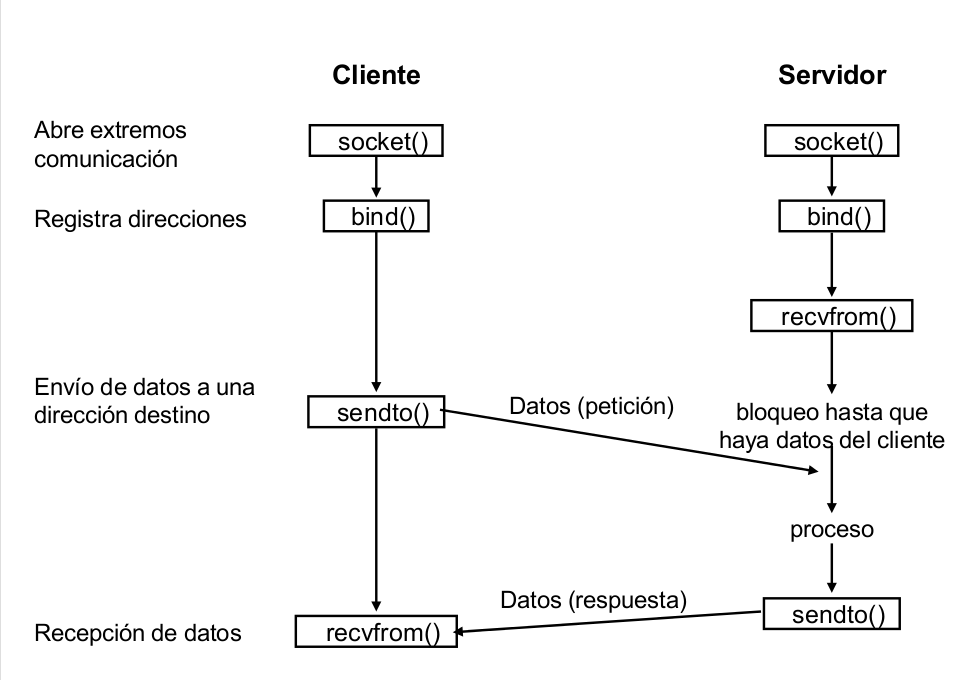
\includegraphics[width=1\textwidth]{img/SocketNoConexion.png}
\caption{Comunicación No Orientada a conexión.}
\label{SocketNoConexion}
\end{figure}
\newpage
\section{Modelos de servicios distribuidos}

La base de este curso es cómo dar servicio a muchos clientes. Si tenemos una web a la que se conectan 10 personas, nos vale con cualquier ordenador, pero ¿Cuánta gente usa google? Ni de coña google tiene un único servidor haciendo todo, tiene que tener los \textbf{servicios distribuidos}. A lo largo de esta sección iremos viendo muchas de las maneras de llevar esto a cabo.

\subsection{RPC - Remote Procedure Calls}
Este modelo se basa en realizar llamadas a funciones como si fueran locales, así el procesamiento de esa función no se realiza en local sino en remoto y nos ahorramos recursos de procesamiento.

Para el funcionamiento de RPCs necesitamos unos componentes intermedios llamados \concept{Stub}. En el siguiente diagrama se entiende perfectamente el funcionamiento de los RPCs.
\begin{figure}[htb]
\centering
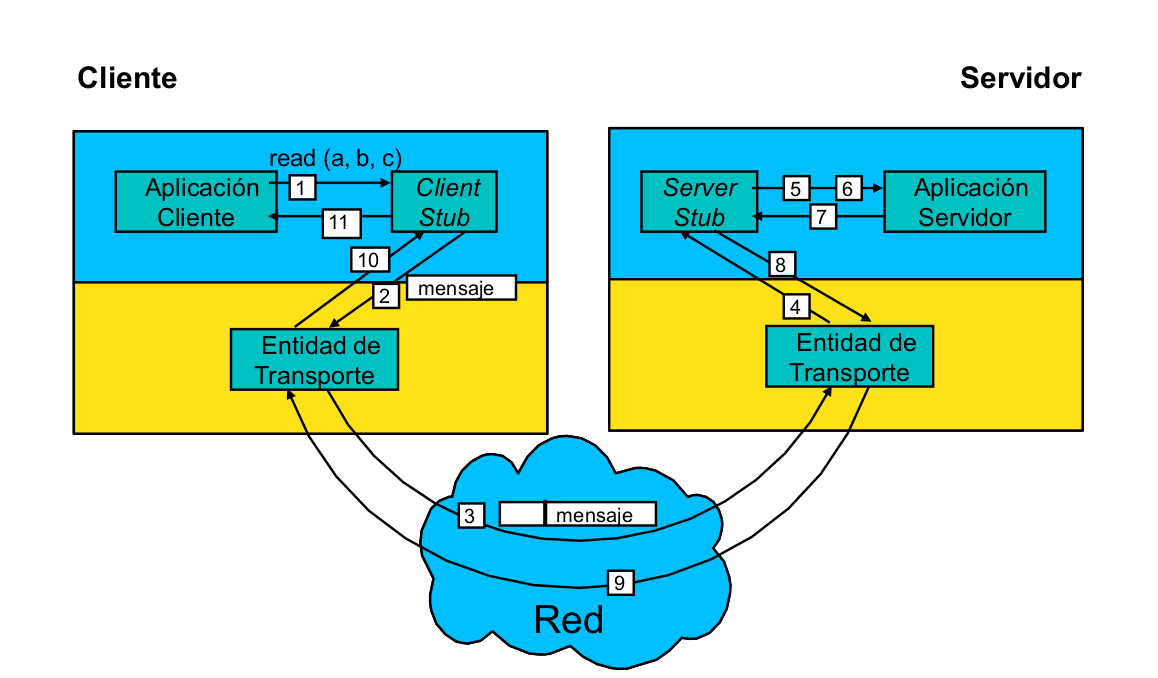
\includegraphics[width=0.9\textwidth]{img/RPC.png}
\caption{Funcionamiento de una llamada RPC.}
\label{RPCimg}
\end{figure}
\newpage

\obs La espera del cliente es \textbf{bloqueante}.

\obs Una ventaja realmente interesante de esto es la transparencia de representación de los datos. RPC (y los stubs intermedios) permiten que un cliente que utiliza Big Endian pueda pasarle los parámetros a una función que se ejecute en un servidor que utiliza Little Endian. Esta \textit{transformación} de los datos de un sistema de codificación al otro se llama \concept{Marshalling} (el codificarlos para enviar) y \concpet{Unmarhsalling} (descodificarlos al recibirlos). Ambos stubs tienen que hacer marshalling y unmarshalling al enviar y recibir mensajes respectivamente.

\paragraph{Problemas de RPC}
\begin{itemize}
	\item No existe el paso de parámetros por referencia.
	\item Hay que conocer de antemano dónde está el servidor exáctamente y en qué puerto escucha.
	\subitem Para saber el puerto en el que el servidor está escuchando, éste tiene que registrarse en un \concept{PortMapper} al que el cliente pregunta por el puerto.
 	\item Tras un \textit{Time Out} No se sabe si la llamada se ha ejecutado o no. Para intentar mitigar este problema en algunos casos, encontramos estrategias distintas en las llamadas RPC:
		\subitem Ejecución Exactamente una vez.
		\subitem Ejecución Como máximo una vez.
		\subitem Ejecución Al menos una vez.\\
	Para solventar esto es necesario también saber si las operaciones son \concept{operaciones de RPC idempotentes} (se pueden ejecutar cualquier número de veces) o no\footnote{Por ejemplo un cálculo $4+4$ lo puedes ejecutar todas las veces que quieras, pero un insert en una base de datos no}.
	\item Es necesaria una representación de datos compartida por los stubs.
	\item Seguridad. ¿Y si el servidor ha sido comprometido y me va a devolver datos que me hagan mal?
\end{itemize}


\paragraph{SUN RPC: } Una de las implementaciones más comunes de RPC es \concept{Sun RPC}. Vamos a estudiarla un poco más en detalle.


Tiene 3 componentes:
\begin{itemize}
	\item \concept{XDR} Lenguaje de definición de tipos de datos. Tiene una sintaxis similar a C, pero es sólo de definición de datos, no de programación
	\item \textbf{Especificación de RPC: } Genera los \textit{stubs} y el fichero de interfaz (para ser incluido al programar)
	\item \textbf{Librería de implementación}
\end{itemize}

Sólo por si interesa, incluimos un esquema de cómo funciona y qué ficheros se generan en la codificación de un servicio utilizando RPC.


\begin{figure}[htb]
\centering
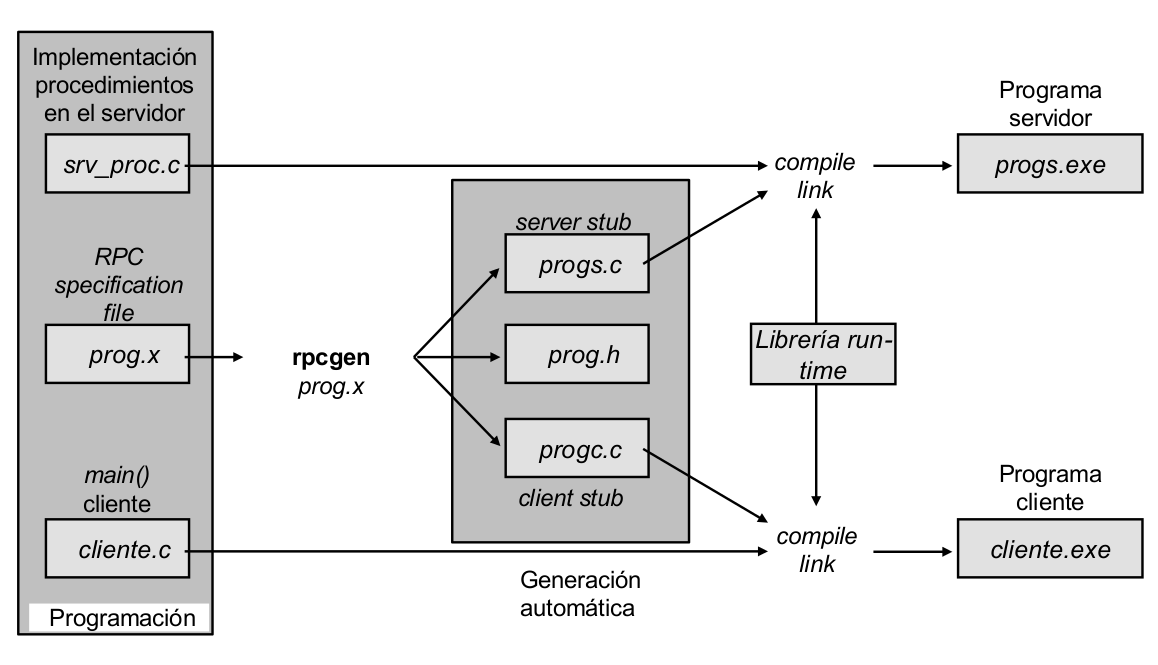
\includegraphics[width=1\textwidth]{img/SUNRPC.png}
\caption{Compilación y generación de código para Sun RPC.}
\label{SunRPC}
\end{figure}

\paragraph{Algunas diferencias entre RPCs}
\begin{itemize}
	\item Parámetros: Aunque en general soporten múltiples parámetros (\concept{Apollo RPC} por ejemplo), Sun RPC sólo tiene un único parámetro, tanto de entrada como de salida (obviamente pueden ser estructuras).
	\item Marshalling: En general lo hace el RPC, aunque en Sun RPC el marshalling que se realiza es mínimo. Es responsabilidad del usuario tener cuidado con eso.
\end{itemize}

Comentamos que Apollo RFC tiene su propio lenguaje de representación de datos, \textit{Network Data Representation} \concept{NDR} (como el XDR de Sun RPC). Apollo tiene también un lenguaje de representación de interfaces \concept{NIDL} (\textit{Network Interface Definition Language}).

\subsection{Web Services (SOAP-WSDL-UDDI)}
Es un modelo de uso de la Web. La idea es tener servidores que ofrecen servicios (localizar geográficamente a través de la IP, ofrecer información de finanzas...) y que cualquiera puede requerir esos servicios. ¿Qué diferencia tiene con RPC? Que en RPC el programador tiene que codificar el lado del servidor y tener conciencia de como funciona, mientras que con los WebServices, el programador que está haciendo un cliente puede utilizar los servicios que le proporciona un servidor que otro programador haya hecho en cualquier otro momento.

Añade un nivel más de transparencia, ya que el programador del cliente no tiene ni idea de cómo funciona el WebService.

La \textbf{función del middleware} aquí es proporcionar funcionalidad para publicar los servicios que ofreces y descubrir los nuevos servicios que vayan surgiendo. Además, tiene que permitir que los servidores soliciten servicios también (multi-\textit{tier}).

\paragraph{Complementos de los Web Services} \concept{OASIS} (Organization for the Advancement of Structured Information Standards) está trabajando (y ha trabajado) en estandarizar una serie de complementos útiles para la mejor utilización de los Web Services y una serie de familia de especificaciones:
\begin{itemize}
\item Complementos:
	\subitem Seguridad.
	\subitem Fiabilidad.
	\subitem Addresing: describir las direcciones de emisor y receptor de un mensaje dentro del propio mensaje.
	\subitem Transaction.
\item \concept{WSRL} - Web Services Resource Framework.
	\subitem WS-Resource (Conjunto de un recurso y un Web Service a través del cual se accede a él.
	\subitem WS-ResourceProperties
	\subitem WS-ResourceLifetime
	\subitem WS-BaseFaults (mecanismo extensible para gestionar errores)
	\subitem WS-ServiceGroup
\end{itemize}

Los WebServices necesitan de 3 protocolos estándares. En el siguiente gráfico se muestran los componentes y protocolos de comunicación utilizados en los WebServices.


\begin{figure}[htb]
\centering
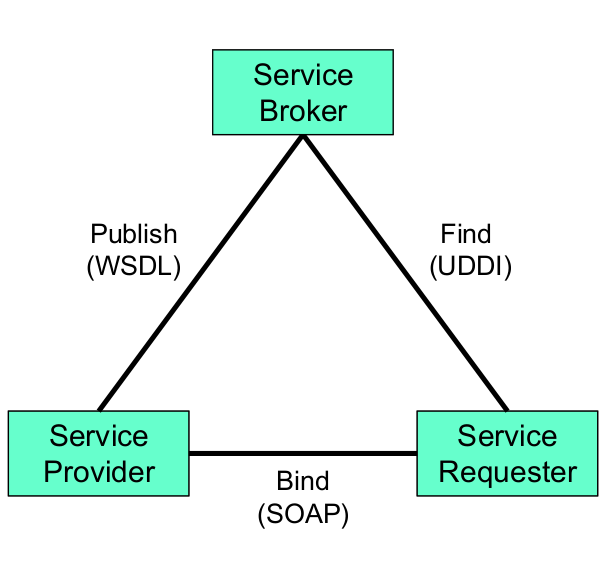
\includegraphics[width=0.9\textwidth]{img/WS.png}
\caption{Componentes de un WS para su funcionamiento.}
\label{WSimg}
\end{figure}


\subsubsection{SOAP}
\begin{defn}[SOAP]
(siglas de Simple Object Access Protocol) Es un protocolo estándar que define cómo dos objetos en diferentes procesos pueden comunicarse por medio de intercambio de datos XML.

Es independiente de la plataforma y el lenguaje de programación y, aunque se puede usar en distintos sistemas de mensajes y sobre distintos protocolos de transporte, su uso principal es transportar RPCs sobre HTTP.
\end{defn}

Un mensaje SOAP es un documento XML ordinario con una estructura definida en la especificación del protocolo. Dicha estructura la conforman las siguientes partes:
\begin{itemize}
\item \textbf{Envelope (obligatoria)}: Raíz que da la estructura, es la parte que identifica al mensaje SOAP como tal.
\item \textbf{Header}: Esta parte es un mecanismo de extensión ya que permite enviar información relativa a cómo debe ser procesado el mensaje. Es una herramienta para que los mensajes puedan ser enviados de la forma más conveniente para las aplicaciones. El elemento "Header" se compone a su vez de "Header Blocks" que delimitan las unidades de información necesarias para el header.
\item \textbf{Body (obligatoria)}: Contiene la información relativa a la llamada y la respuesta.
\item \textbf{Fault}: Bloque que contiene información relativa a errores que se hayan producido durante el procesado del mensaje y el envio desde el "SOAP Sender" hasta el "Ultimate SOAP Receiver"
\end{itemize}

\subsubsection{WSDL}
\begin{defn}[WSDL]
WSDL son las siglas de Web Services Description Language, un formato XML que se utiliza para describir servicios Web.

WSDL describe la interfaz pública de los servicios Web. Está basado en XML y describe la forma de comunicación, es decir, los requisitos del protocolo y los formatos de los mensajes necesarios para interactuar con los servicios listados en su catálogo. Las operaciones y mensajes que soporta se describen en abstracto y se ligan después al protocolo concreto de red y al formato del mensaje.
\end{defn}

Estructura de una declaración WSDL
\begin{itemize}
\item \textbf{definitions}: Elemento raíz que contiene el resto. Define su
nombre y los espacios de nombres que utiliza.
\item \textbf{types}: Tipos de datos utilizados entre cliente y servidor. Usa
W3C XML Schema (XSD) por defecto.
\item \textbf{message}: Declaraciones de mensajes empleados para
peticiones y respuestas y los elementos que los forman.
\item \textbf{portType}: Operaciones soportadas y encadenamiento de
mensajes que implica su ejecución.
\item \textbf{binding}: Modo en que los mensajes se transmiten sobre un
protocolo de RPC, con extensiones específicas para SOAP.
\item \textbf{service}: Contiene la información de la dirección en la que se
localiza el servicio.

\end{itemize}

\subsubsection{UDDI}
\begin{defn}[UDDI]
UDDI son las siglas del catálogo de negocios de Internet denominado Universal Description, Discovery and Integration. El registro en el catálogo se hace en XML. UDDI es una iniciativa industrial abierta (sufragada por la OASIS) entroncada en el contexto de los servicios Web.
\end{defn}

El registro de un negocio en UDDI tiene tres partes:
\begin{itemize}
\item \textbf{Páginas blancas}. Dirección, contacto y otros identificadores conocidos.
\item \textbf{Páginas amarillas}. Categorización industrial basada en taxonomías.
\item \textbf{Páginas verdes}. Información técnica sobre los servicios que aportan las propias empresas.
\end{itemize}
UDDI es uno de los estándares básicos de los servicios Web cuyo objetivo es ser accedido por los mensajes SOAP y dar paso a documentos WSDL, en los que se describen los requisitos del protocolo y los formatos del mensaje solicitado para interactuar con los servicios Web del catálogo de registros.

\paragraph{Ventajas e inconvenientes}

\textbf{Ventajas}
\begin{itemize}
\item Aportan interoperabilidad entre aplicaciones de software independientemente de sus propiedades o de las plataformas sobre las que se instalen.
\item Los servicios Web fomentan los estándares y protocolos basados en texto, que hacen más fácil acceder a su contenido y entender su funcionamiento.
\item Permiten que servicios y software de diferentes compañías ubicadas en diferentes lugares geográficos puedan ser combinados fácilmente para proveer servicios integrados.
\end{itemize}


\textbf{Inconvenientes}
\begin{itemize}
\item Para realizar transacciones no pueden compararse en su grado de desarrollo con los estándares abiertos de computación distribuida como CORBA (Common Object Request Broker Architecture).
\item Su rendimiento es bajo si se compara con otros modelos de computación distribuida, tales como RMI (Remote Method Invocation), CORBA o DCOM (Distributed Component Object Model). Es uno de los inconvenientes derivados de adoptar un formato basado en texto. Y es que entre los objetivos de XML no se encuentra la concisión ni la eficacia de procesamiento.
\item Al apoyarse en HTTP, pueden esquivar medidas de seguridad basadas en firewall cuyas reglas tratan de bloquear o auditar la comunicación entre programas a ambos lados de la barrera.
\end{itemize}

\subsection{REST}
\begin{defn}[REST]
Si bien el término REST se refería originalmente a un conjunto de principios de arquitectura, en la actualidad se usa en el sentido más amplio para describir cualquier interfaz web simple que utiliza XML y HTTP, sin las abstracciones adicionales de los protocolos basados en patrones de intercambio de mensajes como el protocolo de servicios web SOAP.

Es posible diseñar sistemas de servicios web de acuerdo con el estilo arquitectural REST de Fielding y también es posible diseñar interfaces XMLHTTP de acuerdo con el estilo de llamada a procedimiento remoto (RPC), pero sin usar SOAP.

Estos dos usos diferentes del término REST causan cierta confusión en las discusiones técnicas, aunque RPC no es un ejemplo de REST.
\end{defn}

Al trabajar con REST se considera que el sistema se compone de \textbf{recursos}, es decir, elementos que deben ser accedidos en el sistema distribuído y a los que se accede a través de su identificador global \concept{URI}.

Cada acceso a un recurso se contesta con una representación del mismo, que puede incluir enlaces a representaciones relacionadas. Este acceso se basa en el intercambio de mensajes HTTP: GET, PUT, DELETE, POST.

\textbf{REST es una arquitectura, no un estándar.}

\subsection{Comuncación mediante colas de mensajes}

\begin{defn}[MOM]
Message Oriented Middleware.

Es un proceso asíncrono en el que se genera un mensaje, se encola y se sigue lo que se estaba. Como mandar un correo electrónico, que se encola en la bandeja de entrada y tu sigues trabajando.
\end{defn}

Las conexiones en colas de mensajes pueden ser 1-1, 1-N, N-1 y N-M.

\paragraph{Situaciones ideales}
\begin{itemize}
 	\item Conexiones no permanentes y costosas.
 	\item Múltiples servidores procesando mensajes de clientes.
 	\item Llegada de mensajes impredecibles o en ráfagas
 	\item Sistemas de tipo publicación/suscripción.
 \end{itemize}
 \obs Permite balanceo automático de carga en un sistema distribuido. Se pueden procesar los mensajes con prioridades, no necesariamente FIFO.

Vamos a ver algunos ejemplos de gestores de colas.
\subsubsecction{IBM Web Sphere MQ}
Es el MOM más extendido. Es multiplataforma y multiprotocolo.


\concept{IBM Sphere MQ} está formado por
\begin{itemize}
	\item Gestores de colas, encargados de manejar el envío y recepción de los mensajes, además de crear y gestionar el resto de los elementos.

	Tiene una API con
	\subitem Message Queuing Interface (MQI)
	\subitem Application Messagin Interface (AMI)
	\subitem Java Messaging Services (JMS)
	\item Colas de mensajes de múltiples tipos.
	\item Canales de comunicación: Conexiones unidireccionales entre gestores de colas.
\end{itemize}

A continuación mostramos un esquema de funcionamiento de un sistema de mensajería de colas:


\begin{figure}[hbtp]
\centering
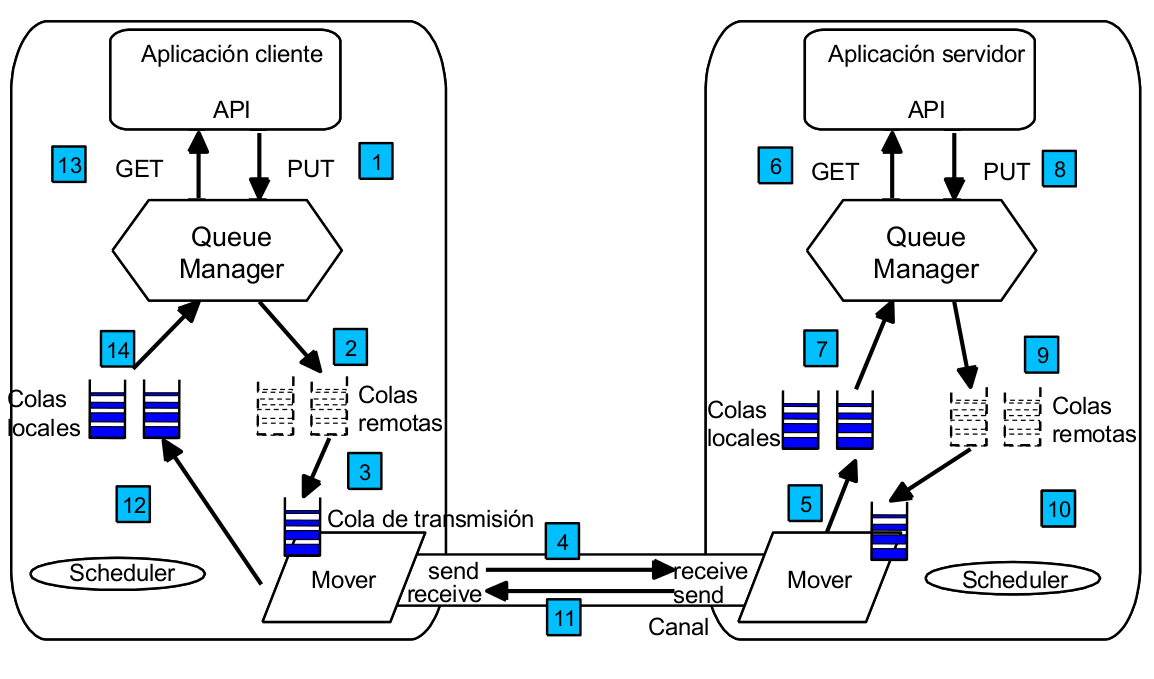
\includegraphics[width=1\textwidth]{img/MOMGen.png}
\caption{Sistema de mensajería de colas.}
\label{MOMGen}
\end{figure}
\newpage

Vemos que se distinguen 3 tipos de colas, las locales (del propio sistema) y las remotas, que el sistema reconoce que pertenecen a otro sistema y entonces el mensaje tiene que ser enviado al sistema al que pertenece la cola remota.

Además de estos 3 tipos de colas (locales, remotas y de transmisión) podemos definir en nuestras colas un par de propiedades: persistentes o temporales (en el almacenamiento de los mensajes) y estáticas (definidas permanentemente) o dinámicas (creadas por aplicaciones). Las colas dinámicas se crean a partir de una cola modelo.

También existen las colas de activación, y de cartas muertas (con mensajes que no se han podido entregar)


En resumen, los tipos de colas pueden ser:
\begin{itemize}
	\item Local - remota.
	\item Persistente - temporal.
	\item Estática - dinámica.
	\item Activación.
	\item Cartas muertas.
	\item Transmisión.
\end{itemize}

\begin{example}
Una de las utilidades de MOM son los servicios de publicación/suscripción. A continuación incluimos un esquema que muestra perfectamente cómo funcionan este tipo de sistemas.


\begin{figure}[hbtp]
\centering
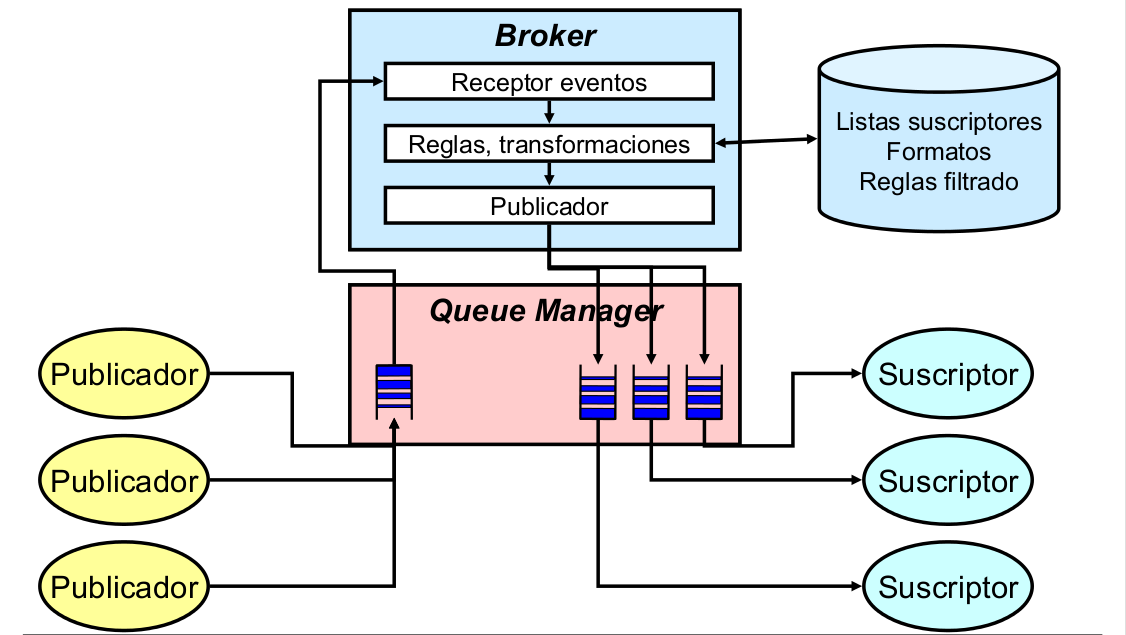
\includegraphics[width=1\textwidth]{img/PubSusc.png}
\caption{Sistema publicador/suscriptor.}
\label{PubSusc}
\end{figure}
\newpage
\end{example}


\section{Services Oriented Architecture SOA}
\subsection{ESB - Enterprise Services Bus}

Extendiendo el modelo de publicador/suscriptor tenemos un ESB. El ESB actúa como proceso centralizador de solicitudes de los clientes (normalmente mensajes o solicitudes de ejecución de acciones tipo RPC – Web Services) para su distribución a los servidores.


\begin{figure}[hbtp]
\centering
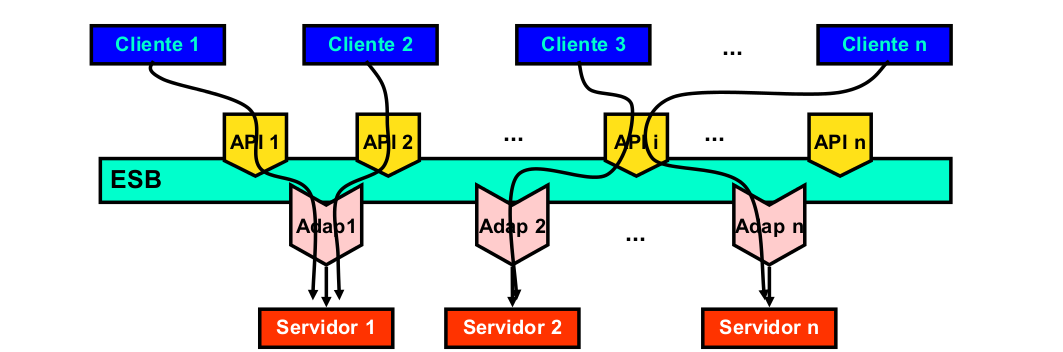
\includegraphics[width=1\textwidth]{img/ESB.png}
\caption{Enterprise Service Bus.}
\label{ESB}
\end{figure}

A continuación, estudiamos las ventajas e inconvenientes que puede tener un sistema como este:
\paragrpaph{Ventajas:}
\begin{itemize}
\item Adaptación rápida en entornos existentes.
\item Flexibilidad. Fácil de adaptar a nuevos requerimientos.
\item Basado en estándares.
\item Existencia de tipos de servicios y APIs predefinidas y listas para su uso.
\item Convierte tareas de programación en configuración (manipulación de datos, por ejemplo).
\item Facilita la gestionabilidad del sistema, al proporcionar un punto único de control para todos los intercambios.
\end{itemize}
\paragrpaph{ Inconvenientes:}
\begin{itemize}
\item Posible punto único de fallo.
\item Fácil saturación del ESB a cargas altas de comunicación.
\item Sin una planificación correcta de APIs y conectores no evita la conexión lógica punto a punto entre clientes y servidores, sólo la física.
\item Requiere más sistemas en ejecución, para soportar el propio ESB.
\item Introducción de un elemento adicional en la cadena de procesamiento, con lo cual el rendimiento se puede ver afectado.
\item Escasas ventajas para entornos sencillos. Estas se ven más en situaciones complejas, con muchos tipos de clientes y servidores.
\end{itemize}

\subsection{RMI - Remote Method Invocation}

Igual que en programación estructurada podíamos ejecutar funciones remotamente (con RPC), con la programación orientada a objetos (POO) también podemos tener localmente una referencia a un objeto remoto y ejecutar métodos del objeto remoto. Para ello es necesario disponer de un middleware espefícico, con unos módulos de comunicación y de referencia remota.


\begin{figure}[hbtp]
\centering
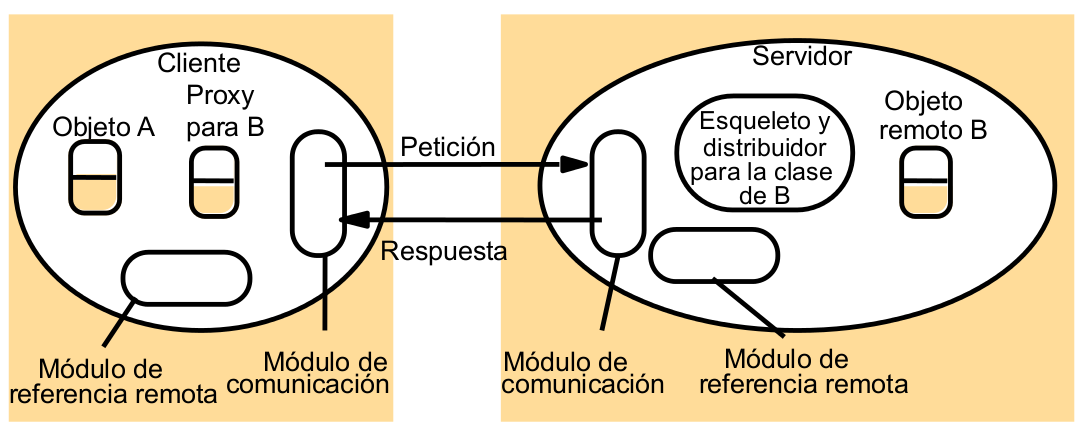
\includegraphics[width=1\textwidth]{img/RMI.png}
\caption{Esquema de funcionamiento de RMI.}
\label{RMI}
\end{figure}

En RMI también es necesario realizar marshalling y unmarshalling. El componente encargado de hacerlo es el esqueleto (del objeto remoto).

El otro componente que merece mención es el módulo de la referencia remota. El objeto que tiene el cliente es una referencia que el módulo de referencias remotas se encarga de traducir la referencia local (a algo remoto) a una referencia remota (al objeto remoto).

Aparte del RMI de Java, existen otras alternativas, como \concept{CORBA} (Common Object Request Broker Architecture) creada por \concept{OMG} (Object Management Group) y \concpet{DCOM} (Distributed Component Object Model) creada por Microsoft.

\subsubsection{OMA}
\begin{defn}[OMA]
Object Management Architecture.

Establece 2 modelos. Un modelo de objetos y uno de referencias.
\end{defn}

Vamos a ver el modelo de referencias.


\begin{figure}[hbtp]
\centering
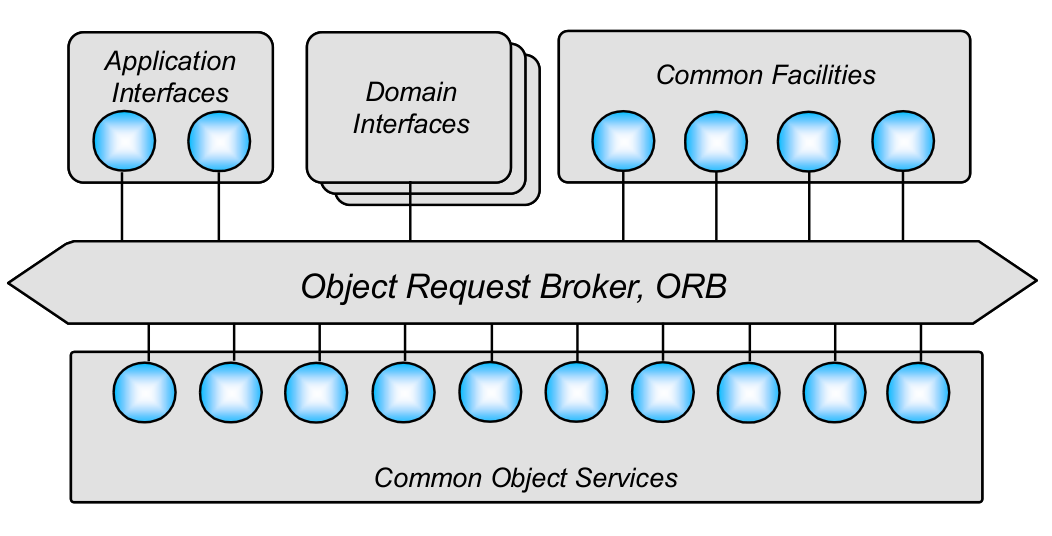
\includegraphics[width=1\textwidth]{img/OMA_Ref.png}
\caption{Esquema de funcionamiento del modelo de referencias de OMA.}
\label{OMA}
\end{figure}

\begin{itemize}
	\item \textit{Object Request Broker, ORB:} Bus de comunicación entre objetos.
	\item \textit{Common Object Services:} Gestión del ciclo de vida, persistencia, resolución de nombres, tiempo, control de concurrencia, seguridad...
	\item \textit{Common Facilities:} Colecciones de componentes, con funciones de tipo general, pero orientados a aplicaciones finales en vez de al sistema.
	\item \textit{Domain Interfaces:} Colección de componentes/objetos comunes específicos para áreas de aplicaciones: comercio electrónico, telecomunicaciones, banca, salud, fabricación...
	\item \textit{Application Interfaces:} Interfaces específicas de aplicaciones concretas.
\end{itemize}

\begin{defn}[ORB]
Object Request Broker → Bus de comunicación entre objetos.

Es un middleware avanzado que es la repera y permite :

\begin{itemize}
	\item Permite llamadas estáticas y dinámicas a objetos. Incluye descubrimiento dinámico de objetos.
	\item Describir las interfaces independientemente del lenguaje de programación. El lenguaje de descripción se llama \concept{IDL}\label{IDL} (Interface Description Language)
	\item Enlace directo de aplicaciones escritas en múltiples lenguajes de alto nivel (no necesariamente orientados a objetos).
	\item Sistema auto-descrito. Genera meta-información consultable dinámicamente.
	\item Soporte de seguridad,transacciones y autenticación de las comunicaciones
	\item Polimorfismo en la ejecución de funciones asociadas a un mismo mensaje.
\end{itemize}
\end{defn}

\begin{defn}[IDL]
Interface description language.
\end{defn}

Del código IDL se crean los stubs necesarios (cliente y servidor\footnote{Los stubs de servidor se llaman \textit{skeletons}}) y los ficheros de definiciones. Además, se genera código fuente del lenguaje elegido, definido en CORBA.

Este es el esquema de desarrollo de un sistema con CORBA.


\begin{figure}[hbtp]
\centering
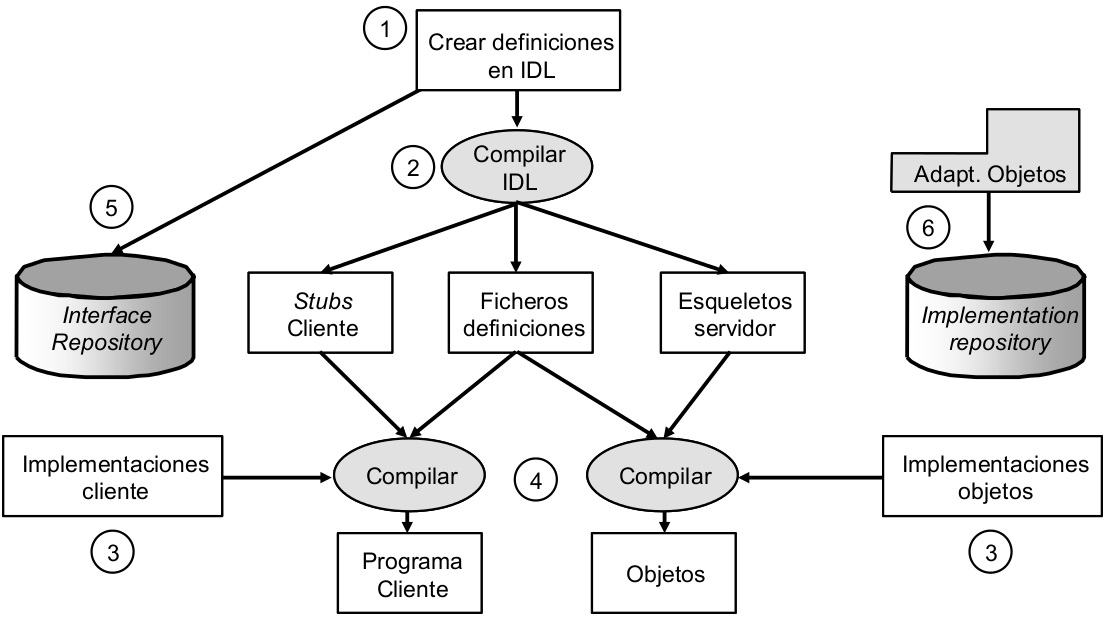
\includegraphics[width=1\textwidth]{img/CORBA.png}
\caption{Esquema del desarrollo de CORBA.}
\label{OMA}
\end{figure}


\subsubsection{Microsoft COM}

\begin{defn}[Microsoft COM]
	Microsoft Component Object Model - Plataforma de objetos de microsoft.
\end{defn}

Esta plataforma de objetos ha ido mejorandose y evolucionando a lo largo del tiempo. Primero fue \concept{DDE} (Dynamic Data Exchange) que mejoró la comunicación entre aplicaciones con \concept{OLE} (Object Linking and Embedding) hasta llegar a \textbf{COM}, con su versión de objetos distribuida \concept{DCOM} y por último, al integrarlo con MTS y MSMQ se ha llegado a \textbf{COM+}

\begin{defn}[MTS]
	Microsoft Transaction Server
\end{defn}

\begin{defn}[MSMQ]
	Microsoft Message Queueing
\end{defn}

\paragraph{Características}
Un objeto COM es un objeto en el mismo sentido que en CORBA,  es independiente del lenguaje de programación y cada objeto tiene una o varias interfaces. Estas interfaces se definen con el Lenguaje de Definición de Interfaces de Microsoft (en inglés \concept{MIDL}). Este lenguaje está basado en el IDL\ref{IDL} del \textit{Distributed Computing Environment} (\concept{DCE}) que utiliza Apollo RFC.

Los sistemas COM se organizan en componentes COM que son módulos binarios (ejecutables o librerías dinámicas). Estos módulos pueden contener uno o varios objetos COM, una interfaz gráfica e incluso otro componente\footnote{Si un componente incluye a otro, el grande se llama componente \textit{ActiveX}}

\paragraph{Funcionalidades}

\begin{itemize}
	\item Transparencia de la localización de los objetos.
	\item Activación de los objetos a distancia (a través del \concept{SCM} (\textit{Service Control Manager})
	\item Seguridad en las comunicaciones (\concept{NTLMP} (\textit{NT Lan Manager Protocol}) y \concept{SAM} (\textit{Security Access Manager})
	\item Descubrimiento dinámico de interfaces (no hay que recompilar todo cuando en un objeto se incluya una interfaz para que podamos utilizarlo)
	\item Reutilización de objetos por agregación y contenencia (\textbf{no herecia})
\end{itemize}


\subsection{Java RMI}
Vamos a ver ahora cómo implementa Java la idea de Remote Method Invocation.

Existe desde Java 1.1 y es más sencillo que CORBA. La arquitectura está basada en 3 niveles: Proxy, Referencia Remota (gestiona las referencias remotas) y Transporte (JRMP - Java remote Method Protocol). Sobre estas 3 capas se construye el cliente y el servidor. Cabe mencionar que el proxy del servidor se denomina esqueleto.

\obs No hay soporte para objetos programados en otro lenguaje (como si permitían las anteriores opciones)

Para programar con Java RMI hay que seguir los siguientes pasos:
\begin{itemize}
	\item Definir las interfaces remotas (extendiendo java.rmi.Remote)
	\item Implementar las clases remotas

	\item Crear proxy y esqueleto compilando con rmi
	\item Crear la aplicación como servidor de la clase remota
		\subitem Crear la instancia
		\subitem Se registra en el servicio de nombres.
	\item Arrancar RMIRegistry y el servidor de la clase remota.
	\item Ya podemos crear clientes con referencias remotas a objetos de la clase implementada.
\end{itemize}

\paragraph{Paso de parámetros}
\begin{itemize}
	\item Todos los parámetros son de entrada salvo el retorno del método.
	\item Admite objetos remotos como parámetros (que obviamente se pasan por referencia)
	\item Admite objetos locales como parámetros sólo si son serializables (que se pasan por valor)
\end{itemize}

\section{Servicios de directorio global}

Reflejan la composición del sistema en todo momento, gestionando el estado de los sistemas que pertenecen a él (pertenencia dinámica) y gestionando las aplicaciones que contiene cada sistema. Estos sistemas tienen que ser Cliente/Servidor para poder ser gestionados por un servicio de directorio global.

Estos servicios se encargan de resolver las transparencia con la ubicación y cada entrada tiene todos los datos asociados al elemento como el estado y la ubicación física\footnote{El servicio de directorio tiene que conocer las ubicaciones físicas y las direcciones para poder ofrecer transparencia a los sistemas que lo utilicen}, aparte de otras variables (estadísticas por ejemplo).


\subsection{Namespaces}
Estos servicios de directorio globales utilizan \concept{namespaces}, es decir, espacios de nombres, de modo que los elementos se pueden reconocer por un nombre en un directorio.

Los nombres deben ser únicos (normalmente asignados por una autoridad dentro del dominio) y no deben contener información de la localización físca, así se garantiza mejor la transparencia a la ubicación.

Este es un ejemplo de un espacio de nombres jerárquico


\begin{figure}[hbtp]
\centering
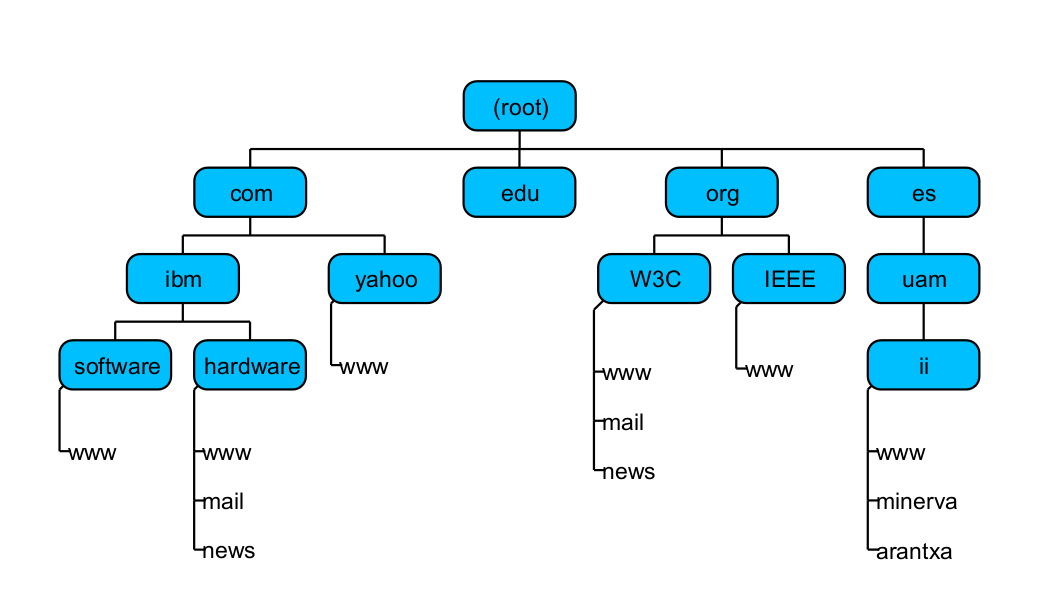
\includegraphics[width=1\textwidth]{img/namespaces.png}
\caption{Espacio de nombres jerárquico.}
\label{namespaces}
\end{figure}

Estos espacios de nombres se pueden utilizar también orientándolo a objetos, de tal manera que cada entrada es una instancia de un objeto. También se pueden tener distintas copias para cada dominio o distribuirlo organizándolo en servicios administrados separadamente ya que el acceso dentro de un dominio sólo requiere un nombre local.

\paragraph{Estándar \concept{X.500}}
Vamos a definir unas cuantas siglas\footnote{Por si acaso no llevamos ya suficientes} necesarias para explicar este estándar

\begin{defn}[XDS]
	APIs de X/Open Direcrory Service
\end{defn}

\begin{defn}[DUA]
	Directory User Agent
\end{defn}

\begin{defn}[DAP]
	Direcroty Access Protocol
\end{defn}

\begin{defn}[DSA]
	Directory System Agent
\end{defn}

\begin{defn}[DSP]
	Direcroty System Protocol
\end{defn}

Los clientes contienen el DUA y se comunicacn con los servidores utilizando DAP.

Los servidores contienen el DSA y se comunican entre servicores utilizando DSP.

Al directorio en sí se accede con las APIs de XDS.


\begin{figure}[hbtp]
\centering
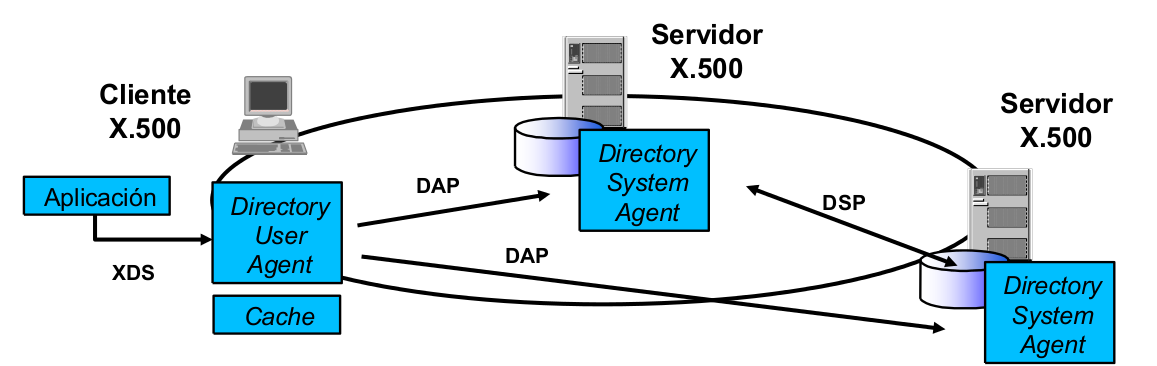
\includegraphics[width=1\textwidth]{img/X500.png}
\caption{Esquema de funcionamiento del estándar X.500.}
\label{X500}
\end{figure}

Existe una alternativa al DAP que es el \concept{LDAP} (\textit{Lightweigth Directory Access Protocol}). Este protocolo no requiere espefícicamente de un directorio X.500, puede utilizarse con \textit{Microsoft Active Directory}.

Esto es un protocolo de comunicaciones, no es una especificación de directorio ni una API de programación. No confundirse.


\subsection{Servicios de tiempo}

Es básico y fundamental que cuando tenemos un sistema distribuido todos los relojes estén perfectamente sincronizados. Para ello existen los servicios de tiempo que vamos a estudiar a continuación.

Sincronizar 2 personas sus relojes es fácil, porque los 2 ven en el mismo instante de tiempo los 2 relojes. 2 ordenadores separados no pueden ver los relojes a la vez, ya que el mensaje con la hora que tiene cada uno tarda en llegar, es por ello que cada ordenador \textbf{mantiene un componente de inexactitud} y que es necesario \textbf{sincronizar periódicamente} cuando ese componente de inexactitud supere un umbral definido\footnote{Tal vez nos podemos permitir 0.01 segundos de desincronización, pero no podemos permitirnos 0.05}

Mantener sincronizado el tiempo es imporescindible para la consistencia y para la \textbf{seguridad}.

Para lograr esta sincronización existen proveedores de tiempo (\concept{timer ticks}) que pueden sincronizar por radio      y actualizar el reloj del administrador de nuestro sistema distribuido. Podemos conectar más de un servidor a estos proveedores.

Una vez tenemos definidos los servidores de nuestro servicio con la hora buena (sincronizados con los timer ticks) el resto de nuestros servidores realizan consultas para sincronizar sus relojes. El formato utilizado es \concept{UTC} (Universal Time Coordinated) que cuenta desde el principio del calendario gregoriano.


\subsubsection{NTP}
¿Y cómo implementamos o utilizamos un servicio de tiempo? Con el \concept{NTP} \textit{Network Time Protocol}, que define una arquitectura para un servicio de tiempo y un protocolo para distribuir la información del tiempo.

\begin{itemize}
	\item Precisión en la sincronización a UTC.
	\item Fiabilidad
	\item Actualizaciones frecuentes (por lo que será necesario que sea resistente a alto nivel de carga)
\end{itemize}

La red de servidores está organizada jerárquicamente. El primer estrato recibe UTC de fuentes  físicas de tiempo (llamadas estrato 0 en wikipedia) y el estrato 2 sincroniza con los primeros. El resto de la red sincroniza con el estrato 2.

Veamos un ejemplo de los cálculos necesarios para sincronizar dos servidores.

\begin{example}
El esquema de la comunicación (intercambio de mensajes) entre los dos servidores que se van a sincronizar es:
\begin{center}
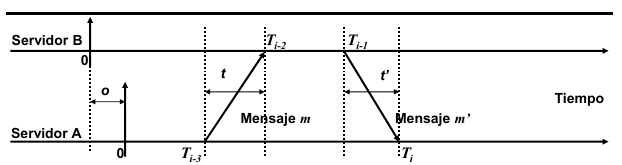
\includegraphics[width=1\textwidth]{img/ntp.png}
\end{center}

Nuestro objetivo es calcular $o$, que es la diferencia de tiempos entre ambos relojes. Observando el esquema, podemos deducir las ecuaciones:
\begin{align}
T_{i-3}+o+t=T_{i-2}\\
T_{i}+o=T_{i-1}+t'
\end{align}
Tampoco conocemos $t$ n $t'$, pues no sabemos el tiempo que ha tardado el mensaje en ser transmitido. Si sumamos las dos ecuaciones y despejamos $o$ de la nueva ecuación nos queda:
\[o=\underbrace{\frac{T_{i-2}+T_{i-1}-T_i-T_{i-3}}{2}}_{o_i}+\frac{t'-t}{2}\]

Así, tenemos $o$ escrito como la suma de un valor conocido más una desviación. Puesto que todos los tiempos son positivos, tenemos que $t+t'>t'-t$ por lo que podemos acotar $o$ mediante:
\[o_i-\frac{\overbrace{t'+t}^{d_i}}{2}\leq o \leq o_i + \frac{\overbrace{t'+t}^{d_i}}{2}\]
\end{example}

\subsection{Seguridad}
Aunque es un tema superimportante (porque en un sistema distribuido se complican las cosas) y tiene un tema dedicado explícitamente a esto, no se va a ver en este curso porque ...

